
\documentclass[11pt]{article}
\usepackage{amsfonts}
\usepackage{amsmath}
\usepackage{common}
\usepackage{color}
\usepackage{float}
\newcommand{\todo}[1]{{\small\color{red}{\bf [*** Todo: #1]}}}
\title{HW 1 Classification}
\author{Justin Chiu \\ justinchiu@seas.harvard.edu \and Demi Guo \\ dguo@college.harvard.edu \and Yuntian Deng \\dengyuntian@seas.harvard.edu }
\begin{document}

\maketitle{}
\section{Introduction}
Sentiment Analysis is a fundamental natural language processing task lying at the root of many text processing systems \citep{nasukawa2003sentiment,miner2012practical,khan2015combining}. 
This task is practically very useful in helping companies or individuals to digest people's overall favorability towards a given product or service. 
Yet it is not that simple as it might appear: even human labelers might not agree over each other's label \citep{liu2010sentiment}; there might be multiple aspects in a sentence with different polarities \citep{lei2016rationalizing}.

In this paper, our goal is to approach this task with various models, from traditional machine learning methods such as Naive Bayes and Logistic Regression, to recent deep learning based methods such as Convolutional Neural Networks \citep{kim2014convolutional} and Recurrent Neural Networks \citep{hochreiter1997long}. We compare the performance of different models, as well as different processing techniques.

\section{Problem Description}
We are given a dataset $\mcD$ = $\{(\boldx_i, y_i)\}_{i=1}^N$, where $\boldx_i$ is a sequence of $l_i$ words: $\boldx_i = \boldx_{i}^1, \boldx_{i}^2, \cdots \boldx_i^{l_i}$ representing text of a customer review, $y_i\in \mcY$ is the corresponding label, usually a ordinal variable such as positive and negative.
We use one-hot encoding to represent words: $\boldx_i^j\in \{0,1\}^{V}$ and 1 is taken only at the word index, where $V$ denotes vocabulary size. Our goal is to infer $P(y_i | \boldx_i)$ on a test dataset given training dataset $\mcD$.


\section{Models}
For brevity, we drop the subscripts of $\boldx_i$, $y_i$ and $l_i$ when no ambiguity arises.
\subsection{Naive Bayes Unigram Classifier}
A Naive Bayes classifier assumes that features are independent of each other given label:
\begin{equation}
    P(\boldx | y) = P(\boldx^1, \boldx^2, \cdots \boldx^{l} | y_i) = \prod_{j=1}^{l}P(\boldx^j | y)
\end{equation}

Then we apply Bayes rule to make a prediction:
\begin{equation}
    P(y | \boldx) \propto P(\boldx | y) P(y)
\end{equation}

We use a categorical distribution with parameters $\boldsymbol{\theta}^y\in \mathbb{R}^V$ to model $P(\boldx^j | y)$:
\begin{equation}
    P(\boldx^j = k | y) = {\theta}^y_k
\end{equation}
where we abuse our notations by using $\boldx^j$ as word index.

Similarly, we use a categorical distribution with parameters $\boldsymbol{\phi}\in \mathbb{R}^{|\mcY|}$ to model $P(y)$:
\begin{equation}
    P(y = k) = {\phi}_k
\end{equation}

The MLE solution of $\boldsymbol{\theta}$ and $\boldsymbol{\phi}$ is just the empirical frequency:
\begin{align}
    &\phi_k = \frac{\# \text{instances with label $k$}}{\# \text{instances}}\\
    &\theta^y_k = \frac{\# \text{words with index $k$ and label $y$}}{\# \text{words with label $y$}}\\
\end{align}

In practice, we usually add pseudocounts to both nominator and denominator to avoid issues with rare or out-of-vocabulary words, and at inference time we do calculations in log space to avoid numerical issues.

\subsection{Logistic Regression Classifier}
In logistic regression, we model $P(y | \boldx)$ as:
\begin{equation}
    P(y|\boldx) = \sigma (\sum_{j=1}^l \boldw^T \boldx^j)
\end{equation}
where $\sigma(\cdot)$ denotes sigmoid function. $\boldw \in \mathbb{R}^V$ are model parameters.
During training we maximize $\sum_{i}\log P(y_i | \boldx_i)$ w.r.t. $\boldw$ by SGD.

\subsection{Bag-of-words Neural Network}
Logistic Regression Classifier can be expressed as a 1-layer neural network. It's straightforward to introduce multiple channels for each word (hence word embeddings) and add a hidden layer to get a 2-layer neural network model.
Since we are still summing the word embeddings thus effectively ignoring word order information, we name this model Bag-of-words Neural Network.

Out model is shown in Fig.~\ref{fig:network_cbow}.
For each word, half of the embeddings come from pretrained vectors and are fixed during training; the other half are randomly initialised and trained. 
We maximize log likelihood with SGD to learn the parameters.
\begin{figure}[H]
    \centering
    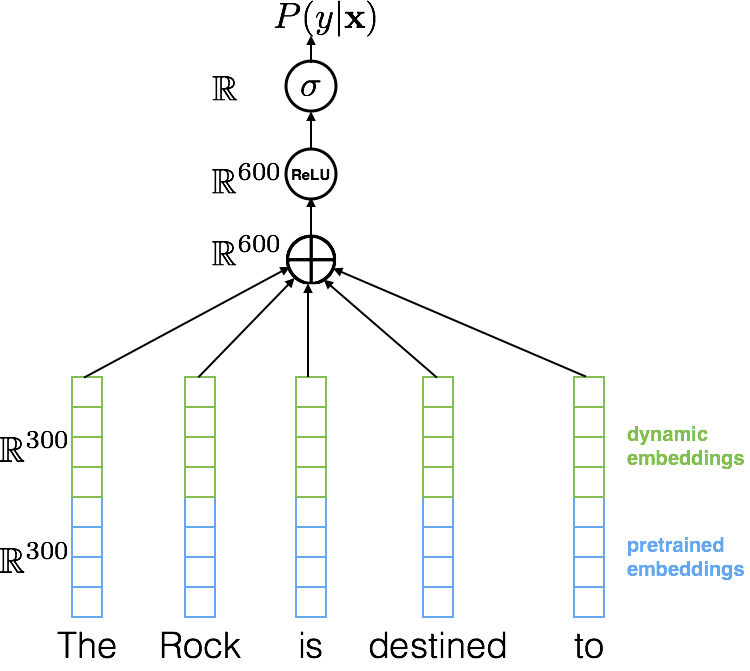
\includegraphics[width=0.6\textwidth]{HW1/writeup/images/network_cbow.png}
    \caption{Bag-of-words Neural Network Architecture}
    \label{fig:network_cbow}
\end{figure}


\subsection{Convolutional Neural Network}
\begin{figure}[H]
    \centering
    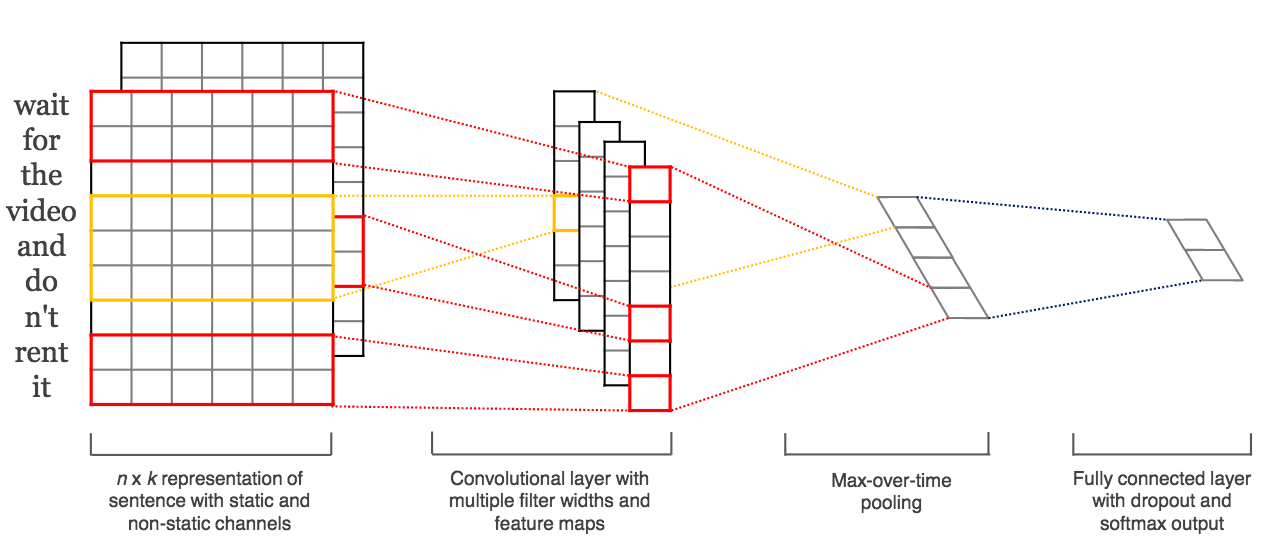
\includegraphics[width=0.6\textwidth]{HW1/writeup/images/network_cnn.png}
    \caption{CNN Architecture. Image courtesy: Kim (2014)}
    \label{fig:network_cnn}
\end{figure}
We adapt the CNN model from \cite{kim2014convolutional} shown in Fig.~\ref{fig:network_cnn}.
We use the same embedding layer as in our Bag-of-word Neural Network model, then we apply 3 convolutional filters with kernel size 3, 4 and 5, each with 100 output channels, and finally we employ max-over-time pooling, dropout, linear projection and sigmoid.
Same to Bag-of-words Neural Network model, we maximize log likelihood with SGD to learn the parameters.

\subsection{Recurrent Neural Network}
We also approach this task with an recurrent neural network. We use LSTM \citep{hochreiter1997long} throughout this paper. We run a forward LSTM, a backward LSTM, and concatenate their final states, project down to a scalar and apply sigmoid to model $P(y|\boldx)$. Training is again performed by maximizing log likelihood with SGD.

\section{Experiments}

We run experiments on the Stanford Sentiment Treebank \citep{socher2013recursive}. Our main results are shown in Table~\ref{tab:results}. \todo{analysis}.

\begin{table}[h]
\centering
\begin{tabular}{llr}
 \toprule
 Model &  & Accuracy \\
 \midrule
 \textsc{NB}    & & N/A  \\
 \textsc{LR}    & & N/A  \\
 \textsc{CBoW}  & & N/A  \\
 \textsc{CNN}   & & N/A  \\
 \textsc{LSTM}  & & N/A  \\
 \bottomrule
\end{tabular}
\caption{\label{tab:results} Main result table. \textsc{NB}: Naive Bayes. \textsc{LR}: Logistic Regression. \textsc{CBoW}: Bag-of-Words Neural Network. \textsc{CNN}: Convolutional Neural Network. \textsc{LSTM}: LSTM model. The hyperparameters of each model type are selected on the validation set.}
\end{table}

We also investigate different strategies of \todo{binarization and other stuff}.

Lastly, we also inspect our learned model qualitatively by \todo{tensorboard visualizations of word embeddings, or learned filters?}
%\begin{figure}
%  \centering
%  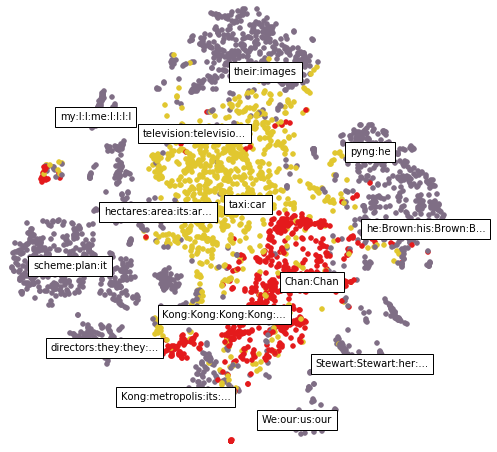
\includegraphics[width=6cm]{cluster_viz}
%  \caption{\label{fig:clusters} Sample qualitative chart.}
%\end{figure}


\section{Conclusion}

In conclusion, we compare different approaches to the classical sentiment analysis problem.

\todo{conclude}

\bibliographystyle{apalike}
\bibliography{writeup}

\end{document}
